\chapter{Solution}
\label{cha:solutioni}
As it's mentioned in the first chapter, the lack of inventor identification information and the non-unique forms of the inventor name make it difficult to do the inventor identification. However, the different forms of the inventor names are usually similar to each other. In addition,  two inventors' names with significant differences show a high probability that they are owned by different people. Therefore, inventor names as good pieces of identification information should be used. The remaining problem is whether two inventors with the same or similar names are the same person or not. In order to solve this problem, some other information such as the assignee, the co-inventors and the location is used. If these kinds of information of the inventors of different patents also show big similarity values, the inventors should be the same person. Nevertheless, some inventors may covers several fields or change the fields and locations. Some patents from the same inventors also show great differences based on different kinds of information.  This problem is solved by using the transitivity. The basic idea of the transitivity is that if two objects are similar to the same object, they are also considered to be similar to each other. This property is performed by using the clustering algorithm. Furthermore, the patent-publication matching can be used as a complementary method to help us to improve the accuracy of the inventor identification. In this chapter, the basic idea of my approach and the approach structure are introduced. Section 3.1 gives an overview of my approach, section 3.2 explains the data structure of my approach and section 3.3 describes the structure of my approach. 

%The lack of the identification information for patent inventors is the reason of inventor identification problem. There are two types of errors for the inventor identification. The first type of error called \emph{lumping error} is to consider different inventors as the same person. The second type of error called \emph{splitting error} is to consider the same person as the different persons. Without the identification information, it's very difficult to say if the two inventors with the same name are the same person or not. Another problem for the inventor dentification is the form of the inventor name. Different forms for the same inventor are allowed for most patent database such as the database from the USPTO and EPO. A simple comparison of the inventor names is not enough to identify the inventor. However, the names of the patent inventor are still good natural identification information. The different forms of the inventor names are usually similar to each other. Although the similar names cannot guarantee the same person, the names with big difference would ensure the owners of these names are different person. Therefore, for most inventor identification approaches, the names are the most important information to be used to distinguish different inventors.  In order to find the inventors with the similar name sare the same person or not. Some other information such as the assignee, technology class and etc. would be used. Nevertheless, the inventor may cover several fields and may also change some information such as the assignee, location and etc. So sometimes the patents from the same person may not have any similarity except the inventor names. As it's explained, the good separation of inventors by using the names leads to the fact that the lumping error is usually smaller than the splitting error. The main problem for the inventor identification is that the inventor with the similar names are the same person or not. My approach gives a solution for the problem by combining the logistic regression and clustering techniques. In this chapter, a general description of my approach for inventor identification would be introduced. In section 3.1, the challenges for the inventor identification and my solutions would be introduced. In section 3.2, the data structure of the patents would be described. In section 3.3, the general structure of the approach would be described. The components and the relationships between the components would also be introduced.
\section{the Overview of the Approach}
This section sketches the inventor identification approach. The patent usually contains a list of inventors. The basic data unit for the inventor identification is the patent plus one of the inventors from the inventor list. For the convenience, the basic data unit uses the same name as the Flemming's raw data name \cite{RePEc:eee:respol:v:43:y:2014:i:6:p:941-955}: the inventor-patent instance. If the patent contains three inventors, there are three inventor-patent instances for this patent. For my approach, some information is used to describe the inventor-patent instances as the features. Between different inventor-patent instances, the similarities based on different features are computed and normalized. Different similarities should have different importance for the inventor identification. The weight sum of these similarities is computed as the global similarity as the formula 3.1. 
\begin{equation}
S_{global}=\sum_i w_i \cdot S_i 
\end{equation}
If the global similarity is larger than a threshold $\theta$, the two inventor-patent  instances are considered from the same person. The weights represent the importance of the feature similarities.
Before implementing this idea, two problems should be solved in advance. The first is the similarity calculation methods of the features. Because different features have different data structures, different similarity calculation methods should be designed for them. The second problem is the weights $w$ and the threshold $\theta$ should be assigned suitable values. Some inventor identification approaches manually adjust the weights or set the same values to all the weights which are not reliable. For my approach, the logistic regression is used to find the suitable values for the weights and the threshold. 
\newline

After the logistic regression, the transitivity is performed by using two different clustering algorithms, the hierarchical clustering and the density-based spatial clustering of applications with noise (DBSCAN). The clustering algorithms group the inventor-patent instances from the same inventors together. These clustering algorithms have different mechanisms to perform the transitivity. The hierarchical clustering uses different methods to calculate the similarities between clusters while the DBSCAN uses a parameter called minimum points (minPts). After the clustering, each cluster is considered to be owned by one inventor. Then a refinement is performed by using the patent-publication matching. For each inventor-patent instance cluster, the related publications for all the patents are extracted from the publication database. The patent-publication matching is based on three different methods to identify the inventor-author linkages. The first method is the non-patent reference matching. If the patent refers to some publications whose authors have the same name as the inventor's, the patent and the publications are matched. The second method is the assignee-affiliation matching, if the patent assignee is same as the publication affiliation and the author and the inventor have the same name, the patent and the publication are matched. The third method is to calculate the similarity between the abstract of the patent and the abstract of the publication, the patent is matched to the publication with the best text similarity and whose author has the same name as the inventor. After the patent-publication matching, the matched author IDs are assigned to the clusters. If two clusters have the same author ID, the clusters will be merged. After the refinement, the final result of the inventor identification is obtained. Compared to other approaches, this approach makes use of a lot of helpful information including the texts of the patents to do the inventor identification. The weights and the threshold are identified by using the logistic regression. In addition, the publication information is also used for the refinement.


%After the logistic regression, a model would be built to identify two persons are the same person or not. However, it's not enough for inventor identification. As it's explained, sometimes the patents from the same person may have no similarities except the names. In order to solve this problem, my approach tries to apply a similarity transitivity by using two clustering algorithm. The basic idea of the similarity transitivity is that if one or more inventor-patent units have global similarity which is larger than the threshold with two different inventor-patent units, the two inventor-patent units would be considered from the same person even their global similarity is less than the threshold. In order to applied the similarity transitivity, the hierarchical clustering and the Density-based spatial clustering of applications with noise (DBSCAN) are be used. After the clustering, another database of the publication would be used to refine the clustering result. For my approaches, after clustering, the inventor-patent units are considered as the same person. For each cluster, the publication of the inventor would be found from the publication database if possible. Because the author from the publication database has an identification information. This information would also be used to see if two clusters contains the same inventor or not. In order to find the publications, three different methods would be used. The first one is to use the patent reference, because some patent would cite the inventor's publications. The second on is to use the assignee of the patent and the affiliation of the publication. If they are same and the inventor name and the author name are also the same, the inventor and the author have a high probability to be same person. The last method is to calculate the similarity between the abstract of the patent and the abstract of the publication, if it's larger than a threshold and the patent inventor and the publication author shares the same name, they are considered as the same person. Because not all the inventors could be assigned to authors, the  matching method only be used to refine the clustering result. 

\section{the Inventor-patent Instance}
\begin{figure}
\centering
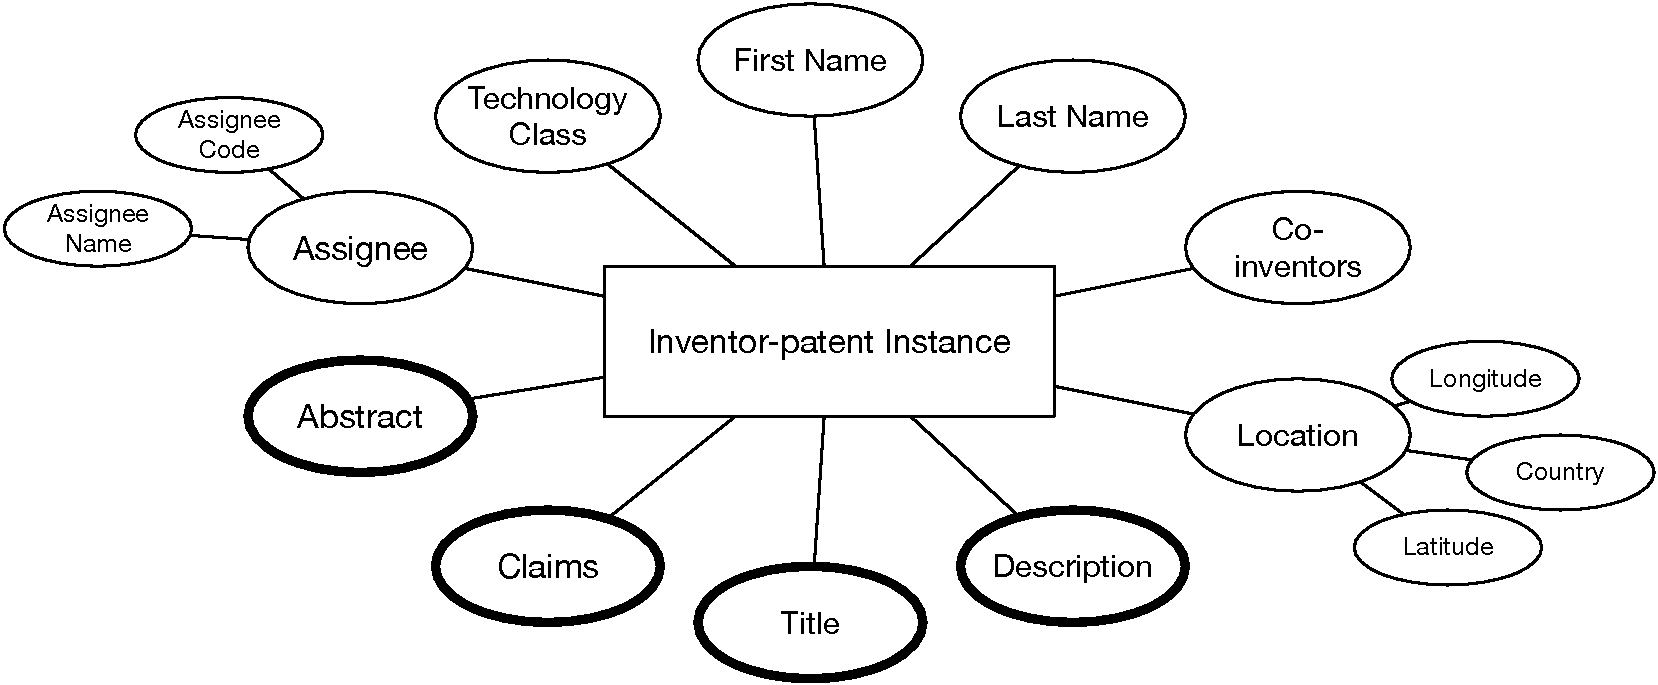
\includegraphics[width=\headwidth]{Patent-inventorUnit.pdf}
\caption{the Inventor-patent Instance}
\end{figure}
The inventor-patent instance is the basic data unit which is processed for my approach. The figure 3.1 shows the data structure of the inventor-patent instance. There are a lot of information in the patent document which can be used as features. Taken Flemming's feature selection \cite{RePEc:eee:respol:v:43:y:2014:i:6:p:941-955} as a reference, ten kinds of information are chosen as features to represent the inventor-patent instance. The ten features are classified into two categories, inventor information features and patent information features. The inventor information  features contain the last name, the first name and the location. The patent information features contain the abstract, the claim, the description, the title, the technology class, the co-inventors and the assignee. The names of the inventors are strings without any punctuation character. The cases of the names' letters are ignored. The middle names are not available for all the inventors, so it's not taken into consideration. The location information contains the longitude, the latitude and the state abbreviations of countries. The title, the abstract, the claim and the description are the texts of the patent document. The technology class is a list of the numeric codes to represent the fields of the patents. The technology classes can be classified into sub-classes and main-classes. Co-inventors are other inventors of the same patent of the inventor-patent instance. The assignee information contains an assign name and an assignee code. Thanks to the free access to the Flemming's database of patents of USPTO from 1975 to 2010, the last name, the first name, the location, the technology class, the co-inventors and the assignee information can be easily extracted from the database. The abstract, the claim, the description and  the title can be extracted by using the patent full-text search engine (PatFt) from the USPTO patent database. This texts are also stored as strings in my approach.

\section{the Approach Structure}
\begin{figure}
\centering
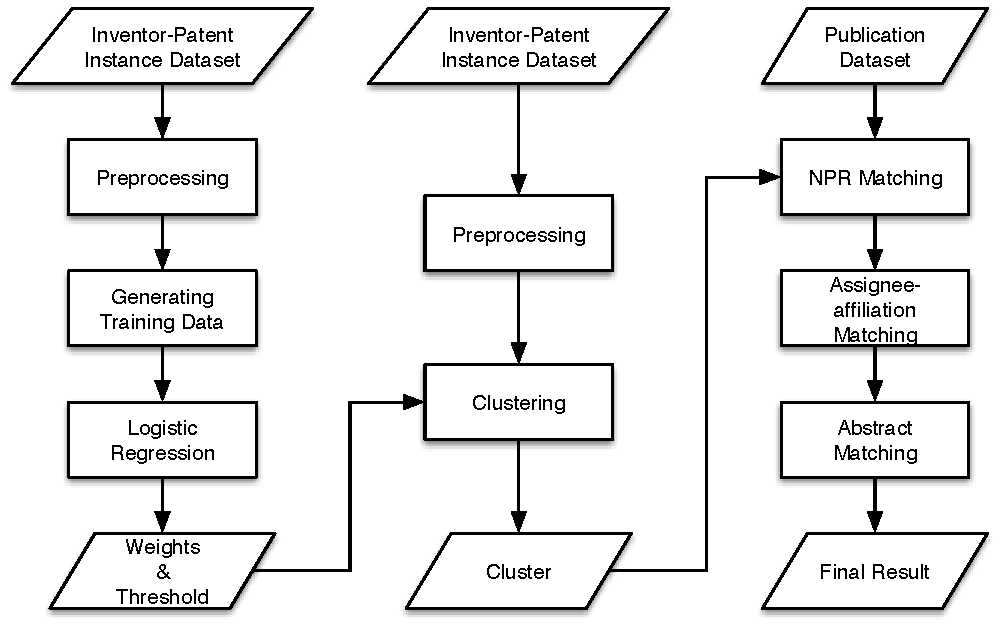
\includegraphics[width=\headwidth]{FlowChart.pdf}
\caption{the Flow Chart of the Approach}
\end{figure}
The figure 3.2 shows the flow chart of my approach. For my approach, an inventor-patent instance dataset with correct identification information for inventors is used as the training dataset. The inventor-patent instance dataset is preprocessed first. The inventor-patent instance information should be extracted from the Flemming's database and the texts of the patents should be extracted by using the patent full-text search engine. After extracting this information, the text mining techniques are applied on the patent texts. These techniques contains removing the stop words, stemming, normalized term frequency calculation and the latent semantic indexing (LSI). The patent text is transformed into the vector representation. The vector representation is used to calculate the similarities between texts. After the preprocessing, the inventor-patent instances are used to generate a training dataset for the logistic regression. The training dataset contains all the pairs of the inventor-patent instances. The logistic regression in my approach is a binary classification. Each pair of inventor-patent instances are used to generate a piece of data in the training data set. This piece of data contains the similarities of the inventor-patent instances based on different features and a label which indicates if the instances are from the same inventor or not. The training dataset is used by the logistic regression to find the suitable values for the weights and threshold. The weights and the threshold are provided to the clustering methods. The weights are used to calculate the global similarity of the two inventor-patent instances.  The global similarity is the measurement to be used to group the inventor-patent instances. The threshold is assigned to some pre-defined parameters  for the clustering algorithms. Usually, for the clustering algorithm, it's difficult to find good values for the pre-defined parameters such as the $K$ for the K-means clustering. For my approach, the logistic regression  helps the clustering to find the values for the pre-defined parameters. When the new inventor-patent instance dataset comes, the same preprocessing method is  applied on it. After the preprocessing,  clustering algorithms are used to group the inventor-patent instances from the same inventor. After that, the publication information from a publication database is used to refine this clustering result. The clusters with the same or similar names of the inventors are chosen as the candidates to be merged. The inventor names are used as the keywords to do the queries in the publication database. The patents for each clusters are matched to the returned publications  by using  three patent-publication matching methods in a serial order. If the patents of the cluster are matched to some  publications, the publication author ID which is matched for the most times is assigned to the cluster. In the end, the clusters with same author IDs are merged. The refined result is used as the final result for the inventor identification.

\newpage
\thispagestyle{empty}
\rule{0cm}{5cm}